\documentclass{beamer}
\usepackage{beamerthemeshadow}
\usepackage{xmpmulti}


\usecolortheme{rose}
\usetheme{Warsaw}

\graphicspath{ {./graphics/} }

\title{Petaluma High School}
\author{Mr. Kelley}
\institute{Petaluma High School}
\date{Spring 2012}

%\newcommand{\dims


\newcommand{ \bigLPic}[2]{
       \includegraphics[scale = .34]<#1>{#2}}

\newcommand{ \bigPPic}[2]{
       \includegraphics[angle = -90, scale = .20]<#1>{#2}}

\newcommand{ \halfnhalfLR}[2]{
       \begin{columns}
       \column{.5\textwidth}
       #1
       \column{.5\textwidth}
       #2
       \end{columns}
}
\newcommand{ \halfnhalfBR}[2]{
       \begin{columns}
       \column{.3\textwidth}
       #1
       \column{.7\textwidth}
       #2
       \end{columns}
}

\newcommand{ \halfnhalfBL}[2]{
       \begin{columns}
       \column{.7\textwidth}
       #1
       \column{.3\textwidth}
       #2
       \end{columns}
}

\newcommand{ \halfnhalfRL}[2]{
       \begin{columns}
       \column{.5\textwidth}
       #2
       \column{.5\textwidth}
       #1
       \end{columns}
}


\begin{document}

\section{Magnetic Fields}

\frame{
       \frametitle{Magnetism}
       \begin{center}
       \includegraphics[scale = .2]<1>{barMagLines}
       \end{center}
}

\frame{
	\frametitle{Magnetism}
	\halfnhalfLR{
	\begin{center}
	\includegraphics[scale = .12]<1>{barMagLines}  
	\includegraphics[scale = .7]<2>{horseMagLines}
	\includegraphics[scale = .5]<3>{ptCharge}
	\includegraphics[scale = .3]<4>{elecDipole}
	\end{center}

	

       }
       {
               \begin{itemize}
               \item<1->{North and South Poles}
               \item<2->{``Dipole"}
               \item<3->{Electric monopoles exist}
               \item<4->{So do electric dipoles}
               \end{itemize}
       }
}
       
\frame{
	\frametitle{Magnetism}
	\begin{center}
       	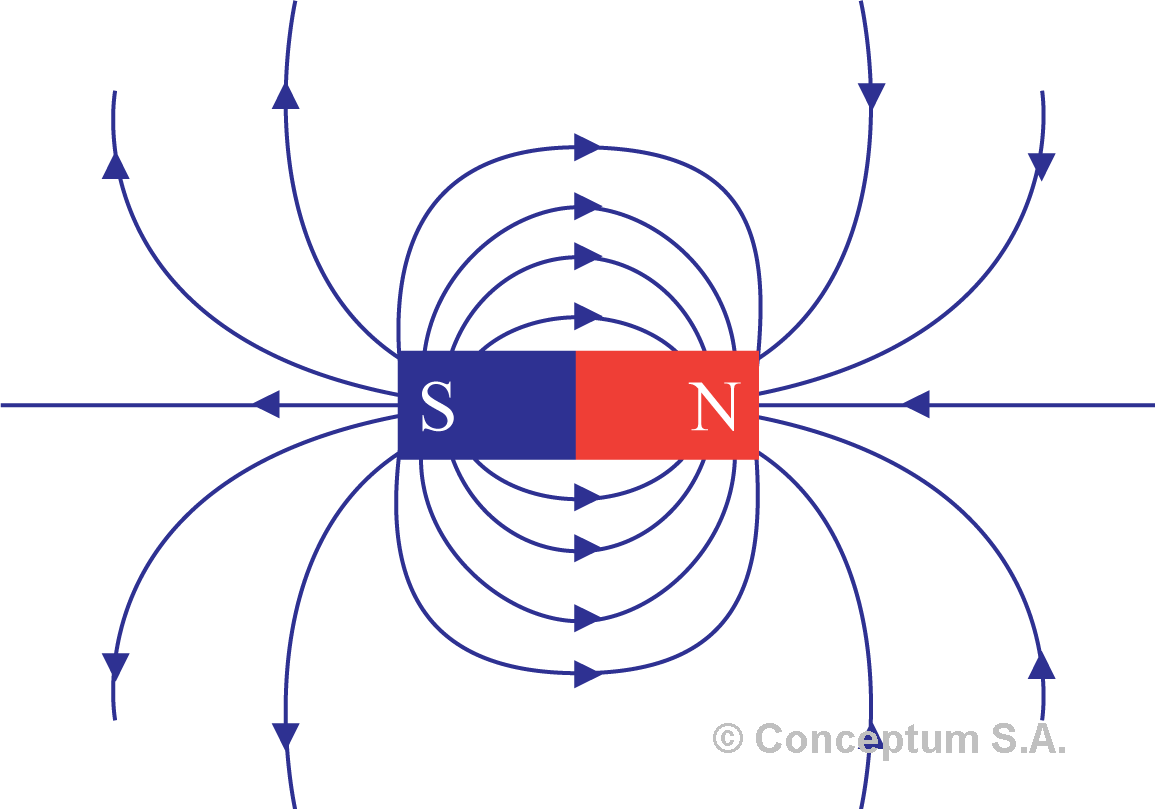
\includegraphics[scale = .2]{barMagLines} \\
	Nobody has \emph{ever} discovered a magnetic monopole. \\
	\pause
	Field lines point \emph{North to South}.
      	 \end{center}
}

\frame{
	\frametitle{Magnetism}
	\halfnhalfLR{
	%\begin{center}
	\includegraphics[scale = .3]<1-4>{likePoles}  \\
	\pause
	Like Poles Repel
	%\end{center}
	}
	{
	%\begin{center}
	\includegraphics[scale = .3]<3-4>{oppPoles}  \\
	\pause
	Opposite Poles Attract
	%\end{center}
	}
}
	
\frame{
	\frametitle{Magnetism}
	\begin{center}
	\includegraphics[scale = .5]<1>{earthDipole}  
	\includegraphics[scale = .3]<2>{messyEarthField}
	\includegraphics[scale = .5]<3>{earthProtectField}
	\end{center}
       }

\frame{
	\frametitle{Source of Magnetic Fields}
	\begin{center}
	\underline{Moving Electric Charge Creates a Magnetic Field.} \\
	\vspace{5mm}
	\pause
	Current is modeled as moving charge, and therefore produces a magnetic field, also known as a ${\bf B}$-field. \\
	\pause
	\vspace{7mm}
	HW: What is the magnetic field due to a straight, current-carrying wire?  What about a loop of wire?\\
	\end{center}
	\vspace{5mm}
	\pause
	Provide at concise and complete explanation using honors-level writing skills (1 paragraph each should be enough if you write well).  Be able to explain the right hand rule for the loop and straight wire for next class. Try Google, Wikipedia, and Kahn Academy.
	\pause
	Or your textbook!
	
	}
       
\frame{
	\frametitle{Lorentz Force}
	\begin{center}
	A charge $q$ moving at a velocity ${\bf v}$ in a magnetic field ${\bf B}$ experiences a force due to the field.
	\pause
	$${\bf F}_B = q {\bf v} \times {\bf B}$$
	\pause
	$$F_B = q v B \sin{\theta}$$
	\pause
	$\theta$ is the angle between the velocity and field vectors. \\
	\pause
	${\bf B}$ is the magnetic field and has units of Teslas (T).
	\end{center}
	}
	
\frame{
	\begin{center}
	\includegraphics[scale = .15]<1>{Tesla} \\
	Nikola Tesla
	\end{center}
}


\frame{
	\frametitle{Lorentz Force}
	Example: \\ 
	An electron traveling to the right at $2.00 \times 10^3 m/s$ enters a uniform magnetic field of magnitude 2.5 T into the page.  What is the magnitude and direction of the force on the electron? \\
	\pause
	$q_e = 1.60 \times 10^{-19} C$
	}

\frame{
	\frametitle{Vectors Again}
	\halfnhalfLR{
	\begin{center}
	Into the Page \\ $$\left.\begin{array}{|cccc|}\hline \bigotimes & \bigotimes & \bigotimes & \bigotimes \\\bigotimes & \bigotimes & \bigotimes & \bigotimes \\\bigotimes & \bigotimes & \bigotimes & \bigotimes \\\bigotimes & \bigotimes & \bigotimes & \bigotimes \\\hline \end{array}\right.$$
	\end{center}

       }
       {
       	\begin{center}
      	Out of the Page \\ $$\left.\begin{array}{|cccc|}\hline \bigodot & \bigodot & \bigodot & \bigodot \\\bigodot & \bigodot & \bigodot & \bigodot \\\bigodot & \bigodot & \bigodot & \bigodot \\\bigodot & \bigodot & \bigodot & \bigodot \\\hline \end{array}\right.$$
     	\end{center}
       }
}

\frame{
	\frametitle{Vectors Again}
	
	\begin{center}
	Cross Products \\
	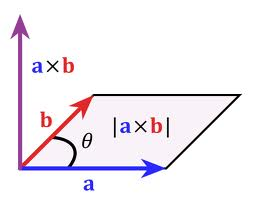
\includegraphics[scale = .6]{crossProd} \\
	The answer to ${\bf a} \times {\bf b}$ is perpendicular to both ${\bf a}$ and ${\bf b}$. \\
	\pause
	This is what the RHR is for. \\
	
	\end{center}
}
       

\frame{
	\frametitle{Vectors Again}
	
	\begin{center}
	Right Hand Rule \\
	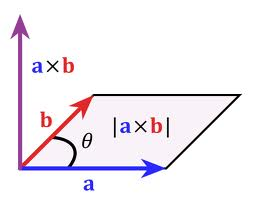
\includegraphics[scale = .4]{crossProd}
	\pause
	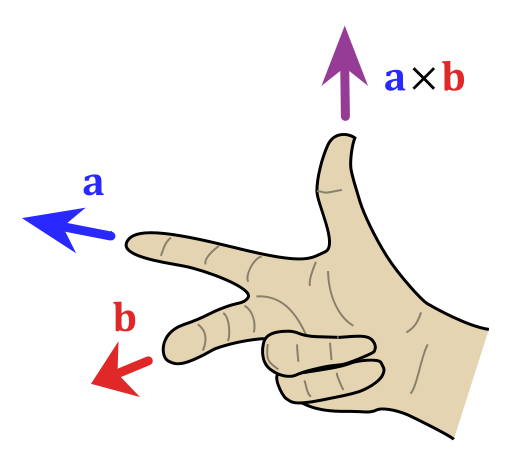
\includegraphics[scale = .2]{rhr}
	
	\end{center}
}

\frame{
	\frametitle{Vectors Again}
	
	\begin{center}
	Right Hand Rule \\
	and Lorentz Force \\
	\end{center}
	 \begin{itemize}
               \item<1->{Straight hand, point fingers in direction of velocity \pause of charged particle.}
               \item<2->{Bend fingers in direction of ${\bf B}$-field.}
               \item<3->{Thumb is now showing you direction of ${\bf F}_B$.}
               \end{itemize}
	
	
}

\frame{
	\frametitle{Magnetism: Important Points}
	
	 \begin{itemize}
               \item<1->{Charges \emph{NOT} \underline{moving} w.r.t. a ${\bf B}$-field do not experience a force due to that field.}
               \item<2->{A \emph{changing} ${\bf B}$-field produces an ${\bf E}$-field, and a changing ${\bf E}$-field produces an ${\bf B}$-field.}
               \item<3->{Stationary charge produces an ${\bf E}$-field, but not a ${\bf B}$-field.}
               \end{itemize}

	
}

       
\end{document}